\chapter{Choosing the Field Before Building the Company}

This chapter comes from a short School of Hard Knocks entrepreneurship interview segment, curated by LazyingArt LLC through Video2Book. The speaker is asked why solar sales stood out as a field to build around. His answer unfolds as a decision sequence: locate a growing industry, separate that growth question from opinion, admit the initial knowledge gap, get close enough to learn, and then decide whether building is justified.

\section{The Opening Question: Why Solar Sales?}

The interviewer begins with the concrete puzzle: what made solar sales stand out? That is the right place to begin. A business does not first appear as an abstract category. It appears as a possible answer to a choice: out of all the fields one might enter, why this one?

The speaker answers by stepping backward. He does not say that he already had a mature theory of solar, energy markets, or sales operations. He places the origin of the decision during his brief time in college:

\begin{equation}
t_0 \approx 2014\text{--}2016.
\end{equation}

At that moment, the question was not yet, ``How do we build the company?'' It was more primitive: where should attention go? Which industries deserve study, contact, and early-career risk?

\section{The Twenty-Year Filter}

The speaker's first filter was a long-horizon growth test. He was looking at emerging industries and asking what would be larger in the next twenty years than it was at the time. As editorial notation for that verbal test, write:

\begin{equation}
S_i(t_0+20) > S_i(t_0),
\end{equation}

where \(S_i(t)\) denotes the scale of industry \(i\) at time \(t\). This is not a formula the speaker gives. It is a compact way to preserve his reasoning: before we ask whether we are expert in an industry, we ask whether the field itself appears to be expanding.

The point is direction, not precision. The transcript does not give market sizes, adoption rates, or expected returns. It gives a practical screen. If the scale of a field is likely to rise, then learning inside that field may compound. If the field is shrinking, even competent work may face a headwind.

\subsection{Question \& Answer}

\paragraph{Question.}
How should we judge an industry when it carries political noise, personal opinions, or cultural disagreement?

\paragraph{Answer.}
The speaker brackets those reactions long enough to ask a colder question: what will be bigger twenty years from now than it is today? Personal preference and personal fit still matter, but they enter after the first screen. In shorthand,

\begin{equation}
G_i =
\begin{cases}
1, & S_i(t_0+20) > S_i(t_0),\\
0, & S_i(t_0+20) \leq S_i(t_0).
\end{cases}
\end{equation}

Here \(G_i\) is not a measured variable from the interview. It is a note-taking device for the speaker's first pass: set aside opinion, inspect the direction of the field, and only then decide whether the field deserves deeper study.

\section{The Candidate Set}

Once the growth test is in place, the speaker names the sectors that came to mind: technology, artificial intelligence, robotics, renewable energy, and crypto. We can record the candidate set as

\begin{equation}
\mathcal{C}
=
\{\text{tech},\ \text{AI},\ \text{robotics},\
\text{renewable energy},\ \text{crypto}\}.
\end{equation}

The modesty of the list matters. It is not a ranking. It is not a research report. It is a remembered scan of fields that seemed likely to grow. Renewable energy matters here because solar sales sits inside that broader category. The speaker is not yet explaining the full mechanics of a solar business. He is explaining how renewable energy entered the field of possible moves.

\section{Ignorance As A Starting Condition}

The next line in the argument is easy to lose, but it is central: the speaker says he did not know much about any of those industries. The entrepreneurial logic does not depend on pretending otherwise. It begins with partial ignorance and then asks how that ignorance can be reduced.

Let \(K_n\) denote working knowledge after \(n\) steps, and let \(F_n\) denote tested fit with the field. The speaker's sequence can be written as the following cautious update rule:

\begin{align}
K_{n+1} &= K_n
+ \Delta K_{\mathrm{study}}
+ \Delta K_{\mathrm{access}},\\
F_{n+1} &= F_n
+ \Delta F_{\mathrm{exposure}}.
\end{align}

Study changes what we know from the outside. Access changes what we learn from proximity. Exposure tests fit. This is a reconstruction, not a quoted formula, but it preserves the spoken order: study the field, get a foot in the door, learn whether it fits, then build around it if the evidence supports that move.

The local derivation is short:

\begin{enumerate}
\item Begin with a candidate industry \(i \in \mathcal{C}\).
\item Apply the growth filter \(S_i(t_0+20) > S_i(t_0)\).
\item If the field passes, invest in study: \(K\) increases through deliberate learning.
\item Seek access: \(K\) increases again because proximity reveals customers, incentives, constraints, and work rhythms.
\item Use exposure to test fit: \(F\) rises only if the field suits the person and the commercial path.
\item Build only after growth, knowledge, access, and fit begin to align.
\end{enumerate}

\section{A Transcript-Derived Process Diagram}

No validated screenshot from this segment contains board work, equations, or a useful diagram. The figure below is therefore not visual evidence from the video; it is a narrow reconstruction of the speaker's verbal sequence.

\begin{figure}
\centering
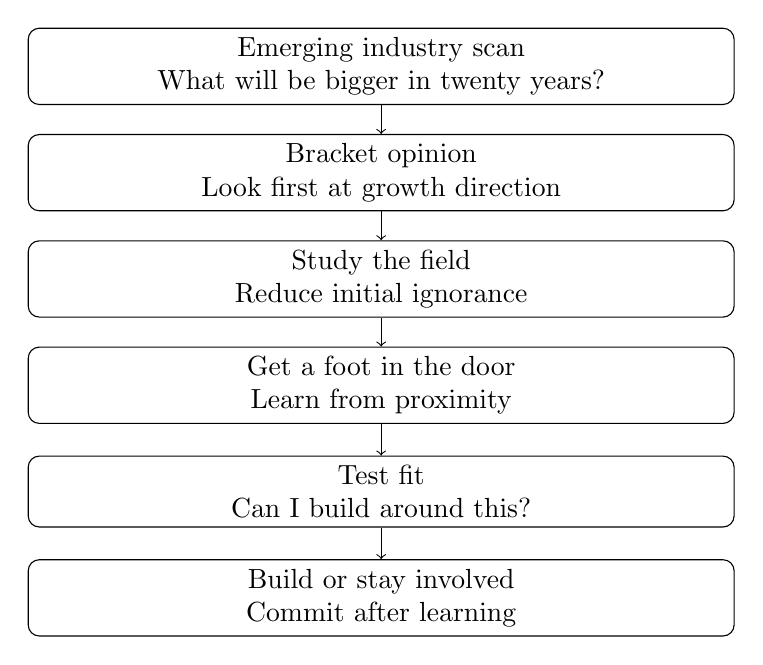
\begin{tikzpicture}[
  box/.style={
    draw,
    rounded corners,
    align=center,
    text width=0.72\linewidth,
    minimum height=0.82cm
  }
]
\node[box] at (0,0) (scan) {Emerging industry scan\\What will be bigger in twenty years?};
\node[box] at (0,-1.35) (filter) {Bracket opinion\\Look first at growth direction};
\node[box] at (0,-2.70) (study) {Study the field\\Reduce initial ignorance};
\node[box] at (0,-4.05) (entry) {Get a foot in the door\\Learn from proximity};
\node[box] at (0,-5.40) (fit) {Test fit\\Can I build around this?};
\node[box] at (0,-6.75) (build) {Build or stay involved\\Commit after learning};

\draw[->] (scan) -- (filter);
\draw[->] (filter) -- (study);
\draw[->] (study) -- (entry);
\draw[->] (entry) -- (fit);
\draw[->] (fit) -- (build);
\end{tikzpicture}
\caption{A transcript-derived reconstruction of the speaker's entry logic. It should be read as an organizing diagram, not as a source screenshot.}
\end{figure}

The diagram deliberately stays vertical and narrow. For a pocket-size page, the important thing is not visual complexity but preserving the sequence: growth scan, opinion bracket, study, access, fit test, and only then commitment.

\section{A Worked Example: Renewable Energy As Doorway}

Now specialize the candidate industry to renewable energy:

\begin{equation}
i = \text{renewable energy}.
\end{equation}

The transcript supports only the first directional claim: renewable energy was one of the fields the speaker believed could be larger over a long horizon. In our notation, the screen is

\begin{equation}
S_{\mathrm{renewable}}(t_0+20)
>
S_{\mathrm{renewable}}(t_0).
\end{equation}

Passing that screen does not yet mean, ``start a company.'' It means the field is worth approaching. The next question is whether there is an accessible doorway. Solar sales can play that role because it puts a person near customers, objections, incentives, installation economics, and demand signals.

A compact way to summarize the reconstructed opportunity test is

\begin{equation}
O_i
\approx
D_i + A_i + L_i + F_i,
\end{equation}

where \(D_i\) is growth direction, \(A_i\) is access, \(L_i\) is learnability, and \(F_i\) is fit. The approximation sign is doing important work. This is not arithmetic, and the speaker does not claim to compute an opportunity score. The notation simply keeps the pieces visible. Growth without access remains distant. Access without learning remains shallow. Learning without fit may not become a durable business.

\section{From Involvement To Building}

The closing beat broadens the lesson. The speaker says it did not have to be starting a business. It only had to be involvement in those industries. That line prevents the chapter from turning the story into an instant-founder myth.

We can write the commitment ladder as

\begin{align}
\text{Stage 1} &: \text{enter a growing field},\\
\text{Stage 2} &: \text{learn through study and proximity},\\
\text{Stage 3} &: \text{test personal and commercial fit},\\
\text{Stage 4} &: \text{build, operate, or remain strategically involved}.
\end{align}

The order is the lesson. The speaker did not begin with complete knowledge of renewable energy. He began with a growth hypothesis, then looked for a way to become involved. Building a solar sales company becomes intelligible only after those prior steps: identify the expanding field, get close, learn, test fit, and then build around the opportunity if the evidence keeps improving.

\section{Summary}

The chapter's spine is a disciplined entry sequence. Around 2014--2016, the speaker looked for industries that seemed likely to be larger twenty years later. He separated that trend question from personal or political preference, named several candidate sectors, admitted limited knowledge, and treated study plus access as the way to learn.

Solar sales mattered because it was a doorway into renewable energy, not because the entire business was obvious at the start. The source gives us no board mathematics or visual diagrams, so the notation here is deliberately light: it is a structured companion to the interview, not a replacement for it. The durable principle is staged commitment: choose the field before choosing the company, get close enough to learn, test fit, and build only when growth, access, learnability, and fit begin to reinforce one another.